\chapter{提案手法}
\label{ch:app}
\quad

本研究で活用する手法,それに対するアプローチをはじめ,テーブルの構造や内容などのシステム設計を示す.
また,WordNet データベースとの連携方法に加えて,ドキュメントをどのようにカテゴライズするかを具体的に示す.

\section{システム設計}
\label{sec:app_design}
本研究のシステムのバックエンドに当たる部分を具体的に示す.
\subsection{データベース設計}
\label{subsec:table}

本研究で使用するテーブルには3種類ある.図 4.1に,これらを表す ER 図を示す.

\paragraph{Word テーブル}
Wordnet データベースの単語が格納されており,主キーである整数型の wordid カラム,言語を表す文字列型の lang カラム,単語名を表す文字列型の lemma カラムによって形成されている.

\paragraph{Synset テーブル}
WordNet データベースに含まれる単語の定義が格納されており,主キーである文字列型の synset カラム 定義名を表す name カラムによって形成されている.

\paragraph{Sense テーブル}
前述した2つのテーブルの中間テーブルであり,Word テーブルとの外部キーである wordid カラム,Synset テーブルとの外部キーである synset カラム,言語を表す文字列型の lang カラムによって形成されている.

\clearpage

\begin{figure}[h]
    \label{fig:er_diagram}
    \centering
    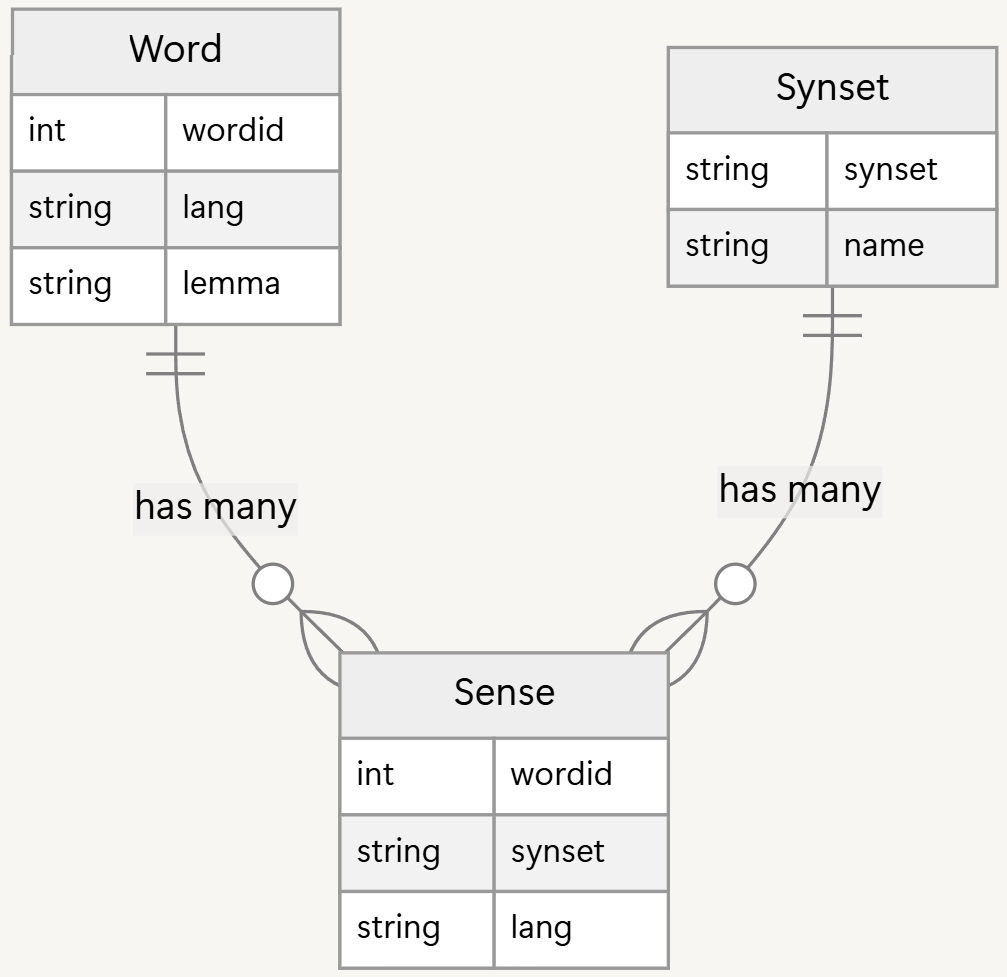
\includegraphics[scale = 0.4]{img/er_diagram.png}
    \caption{データベースの ER 図}
  \end{figure}

\subsection{モデル設計}
\label{subsec:model}

Ruby on Rails にはモデルという概念があり,データベースの内容をモデルとして定義することで,CRUD 処理を始めとしたバックエンドでのデータベースのやり取りを効率的にすることができる.
本研究では第~\ref{subsec:table}節で示したテーブルをモデルとして定義し,整合性等のデータベースレベルの具体的なプロパティを設定する.

\paragraph{Word モデル}
単語に関する情報が格納されている.Sense モデルと一対多の関係で,複数のSense モデルへのリレーションを持っており,Sense モデルを経由して,Synset モデルへのリレーションを辿ることで,単語からその定義を取得する.
場合に応じて適切な言語のレコードを活用するため,言語での絞り込みをするスコープを持つ.

\paragraph{Synset モデル}
単語の定義に関する情報が格納されている.主キーは文字列型の synset カラムである.Sense モデルと一対多の関係で,複数の Word モデルへのリレーションを持っており,Sense モデルを経由して,Word モデルへのリレーションを辿ることで,特定の定義をもつ単語を取得する.
Wordモデルと同様に,言語での絞り込みをするスコープを持つ.

\paragraph{Sense モデル}
Sense モデルは,上記の2つのモデルそれぞれと一対多のリレーションを持っている.synset カラムと wordid カラムが格納されており,それらを外部キーとして使用している.カラムと2つのモデルの双方向に紐づける役割を担う.単語と定義間で実行される処理は,Sense モデルを経由する.

\section{提案する手法 ・ アプローチ}
\label{sec:app_method}

本研究での手法の流れを以下に示す.始めに,カテゴライズしたいドキュメントファイルをシステムにアップロードする.その後,ファイルに対して OCR 処理をして,内容の単語群を取得する.
OCR と親和性のある代表的なプログラミング言語として Python が挙げられるが,http リクエストによって言語を問わず簡単に利用できる点や,OCR 処理に対するオプションの豊富さから,Google Vision API を本研究で使用する.
その後,WornNetデータベースと連携し,単語ごとの定義を取得する. WordNet は日本語,英語双方に対応した対規模な語彙データベースであるため,言語の入り混じったドキュメントに対しても問題なく処理をすることができるため,対応可能な語彙の量と汎用性を加味し,本研究で使用する.
各々の定義を元に単語がどのカテゴリに属するかを判別し,単語ごとにラベリングをする.ラベリング結果から,最終的なドキュメントのカテゴリを決定する.なお,各々のカテゴリに関しては,WordNet の Synset モデルにカテゴリ名を入力し,単語群を取得する方法で用意している.


\subsection{ドキュメントファイルをアップロード}
\label{subsec:app_upload}

Web上で動くRuby on Railsのシステムに対して,カテゴライズしたいドキュメントのファイルをアップロードする.
ファイルのアップロード用のアップローダークラスを定義し,詳しいオプションの設定をする.
アップロードされた画像ファイルのインスタンスをサービスクラスに渡し,OCR 等の処理をする.
上記の処理の流れをソースコード4.1に示す.

\begin{lstlisting}[language=HTML, caption=フロントエンドの ERB]
    <%= form_with(model: @document, url: '/', method: :post,
        multipart: true) do |form| %>
        <div class="form">
            <%= form.file_field :document_file %>
        </div>
        <%= form.submit 'アップロード' %>
    <% end %>
\end{lstlisting}

\subsection{OCRによってドキュメントの内容を取得}
\label{subsec:app_ocr}

Google Vision API の OCR 機能を用いて,ドキュメントの内容を取得し,単語ごとに分割する.
本研究では,まず OCR を実行するために Google Vision API を活用し,外部サービスと連携するためのサービスクラスを設計する.
このサービスクラス内で,API リクエストの送信処理やレスポンスの解析処理を行う.

まず VisionOcrService クラスのインスタンスを初期化する際に,画像認識のための ImageAnnotator::Client インスタンスを生成し,OCR を行う画像のパスを取得する.
次に,指定された画像ファイルの内容をバイナリ形式で読み込み,Vision API にリクエストを送信する.
API のレスポンスは,テキスト認識結果を保持するオブジェクトとして返される.このオブジェクト内から,OCR 結果として取得した文字列データをプロパティから抽出し,
単語の配列として整形する.処理の最終段階では,API 通信時のエラー処理として,ネットワークエラーや API 側の制限に伴う例外処理を行い,適切なエラーメッセージをログに記録することで,システムの信頼性を向上させる.
詳細な処理の流れをソースコード4.2に示す.

\begin{lstlisting}[language=Ruby, caption=Ruby による OCR の実装]
    require "google/cloud/vision/v1"

    class VisionOcrService
        def initialize(image_path)
            @image_path = image_path
            @vision = Google::Cloud::Vision::V1::
            ImageAnnotator::Client.new
        end

        def detect_text
            image_content = File.binread(@image_path)
            response = @vision.text_detection(image: {content:
            image_content})

            response.resources.flat_map do |res|
            res.text_annotations.map(&:description)
        end

        rescue StandardError => e
            Rails.logger.error "Vision API Error: #{e.message}"
            []
        end
    end
\end{lstlisting}

\subsection{それぞれの単語の定義の取得}
\label{sebsec:app_synset}

OCR によって取得した単語に対し,WordNet のデータベースを用いて定義を取得する.まず OCR の結果を配列形式でインスタンス変数に格納し,その後,分析プロセスを開始する.

具体的には,まず単語リストに対して,WordNet の Word テーブルから該当するエントリを検索し,関連する定義情報を取得する.
定義情報が見つからない場合は,"カテゴリ無し" として処理する.これらの処理は,OCR 結果のすべての単語に対して適用される.
最終的に,Synset テーブルの一覧をもとに,文書のカテゴリを判定するためのデータが整えられる.詳細な処理の流れをソースコード4.3に示す.

\begin{lstlisting}[language=Ruby, caption=ActiveRecord による WordNet との連携]
    class AnalyzeController < ApplicationController
        before_action :set_words, only: [:analyze]

        def analyze
            @category_labels = Hash.new(0)

            @words.each do |word|
                analyze_word = Word.includes(:synsets).find_by(lemma:
                word)
            return showNoCategoryError if analyze_word.nil?

            result_words = analyze_word.synsets.pluck(:name)
            current_labels = label_category(result_words)

            current_labels.each do |category, count|
                @category_labels[category] += count
            end
        end
            @result_category = get_category(@category_labels)
        end

        private
        def set_words
            @words = @ocr_response
        end
    end
\end{lstlisting}

\subsection{単語ごとにカテゴライズ,ラベリング}
\label{sebsec:app_categolize}

取得した単語の定義を基に,文書を適切なカテゴリに分類するためのラベリングを行う.
カテゴライズ処理では,WordNet から取得した Synset 情報をもとに,どの単語がどのカテゴリに属するかを決定する.システムは,各 Synset を解析し,それがどのカテゴリに該当するかを判別する.
この過程では,単語リストとカテゴリのマッピングをハッシュ形式で保持し,各カテゴリのカウントを増加させることで,どのカテゴリが最も関連性が高いかを測定する.

具体的には,単語を一意の集合として扱い,カテゴリごとの Synset 情報を取得し,対応するカテゴリラベルの数をカウントする.
これにより,文書内の単語がどのカテゴリに属しているかを判別し,最終的な文書のカテゴリ決定へと繋げる.詳細な処理の流れをソースコード4.4に示す.

\begin{lstlisting}[language=Ruby, caption=カテゴリのラベリングメソッド]
    def label_category(words)
        words_set = words.to_set

        categories = Category.all
        words_with_synsets = Word.where(lemma:
        categories.pluck(:value)).includes(:synsets)

        synsets_by_category = words_with_synsets
            .each_with_object({}) do |word, hash|
            hash[word.lemma] = word.synsets.map(&:name)
        end

        categories.each_with_object({}) do |category,
        category_labels|
            synset_names = synsets_by_category[category.value] || []
            label_count = synset_names.count { |name| words_set
                .include?(name) }
            category_labels[category.value] = label_count
        end
    end
\end{lstlisting}

\subsection{ラベリング結果から文章のカテゴリを決定}
\label{subsec:app_classify}

ラベリングされた結果をもとに文書の最終的なカテゴリを決定する.すべての単語に対してカテゴリが割り当てられた後,カテゴリごとのラベルカウントを集計し,最も多く出現したカテゴリを文書の主要カテゴリとして選定する.

まず受け取ったラベルデータのハッシュを解析し,カウント数が最大のカテゴリを特定する.
この処理の際,カテゴリが全く見つからなかった場合には,エラーをスローし,適切なメッセージを表示することで,未分類の文書に対する処理を明確化する.
最終的に,識別されたカテゴリは,文書全体のカテゴリとして出力される.詳細な処理の流れをソースコード4.5に示す.

\begin{lstlisting}[language=Ruby, caption=文書のカテゴリを決定するメソッド]
    def get_category(labels)
        max_label = labels.max_by { |_, value| value }
        if max_label[1] == 0
            showNoCategoryError
        else
            return max_label[0]
        end
    end

    def showNoCategoryError
        return 'no category'
    end
\end{lstlisting}
